% Created 2024-11-30 Sat 20:20
% Intended LaTeX compiler: pdflatex
\documentclass[11pt]{article}
\usepackage[utf8]{inputenc}
\usepackage[T1]{fontenc}
\usepackage{graphicx}
\usepackage{longtable}
\usepackage{wrapfig}
\usepackage{rotating}
\usepackage[normalem]{ulem}
\usepackage{amsmath}
\usepackage{amssymb}
\usepackage{capt-of}
\usepackage{hyperref}
\usepackage[polish]{babel}
\usepackage[T1]{fontenc}
\usepackage[utf8]{inputenc}
\selectlanguage{polish}
\usepackage{caption}
\usepackage{booktabs}
\captionsetup{labelfont=bf}
\usepackage{float}
\usepackage{svg}
\usepackage[a4paper, total={6in, 10in}]{geometry}
\author{Piotr Karamon}
\date{02.12.2024r.}
\title{Laboratorium 8 - Active Objectasynchroniczne wykonanie zadań w puli wątków przy użyciu wzorców Executor i Future}
\hypersetup{
 pdfauthor={Piotr Karamon},
 pdftitle={Laboratorium 8 - Active Objectasynchroniczne wykonanie zadań w puli wątków przy użyciu wzorców Executor i Future},
 pdfkeywords={},
 pdfsubject={},
 pdfcreator={Emacs 29.2 (Org mode 9.7.11)}, 
 pdflang={Polish}}

% Setup for code blocks [1/2]

\usepackage{fvextra}

\fvset{%
  commandchars=\\\{\},
  highlightcolor=white!95!black!80!blue,
  breaklines=true,
  breaksymbol=\color{white!60!black}\tiny\ensuremath{\hookrightarrow}}

% Make line numbers smaller and grey.
\renewcommand\theFancyVerbLine{\footnotesize\color{black!40!white}\arabic{FancyVerbLine}}

\usepackage{xcolor}

% In case engrave-faces-latex-gen-preamble has not been run.
\providecolor{EfD}{HTML}{f7f7f7}
\providecolor{EFD}{HTML}{28292e}

% Define a Code environment to prettily wrap the fontified code.
\usepackage[breakable,xparse]{tcolorbox}
\DeclareTColorBox[]{Code}{o}%
{colback=EfD!98!EFD, colframe=EfD!95!EFD,
  fontupper=\footnotesize\setlength{\fboxsep}{0pt},
  colupper=EFD,
  IfNoValueTF={#1}%
  {boxsep=2pt, arc=2.5pt, outer arc=2.5pt,
    boxrule=0.5pt, left=2pt}%
  {boxsep=2.5pt, arc=0pt, outer arc=0pt,
    boxrule=0pt, leftrule=1.5pt, left=0.5pt},
  right=2pt, top=1pt, bottom=0.5pt,
  breakable}

% Support listings with captions
\usepackage{float}
\floatstyle{plain}
\newfloat{listing}{htbp}{lst}
\newcommand{\listingsname}{Listing}
\floatname{listing}{\listingsname}
\newcommand{\listoflistingsname}{List of Listings}
\providecommand{\listoflistings}{\listof{listing}{\listoflistingsname}}


% Setup for code blocks [2/2]: syntax highlighting colors

\newcommand\efstrut{\vrule height 2.1ex depth 0.8ex width 0pt}
\definecolor{EFD}{HTML}{000000}
\definecolor{EfD}{HTML}{ffffff}
\newcommand{\EFD}[1]{\textcolor{EFD}{#1}} % default
\newcommand{\EFvp}[1]{#1} % variable-pitch
\definecolor{EFh}{HTML}{595959}
\newcommand{\EFh}[1]{\textcolor{EFh}{#1}} % shadow
\definecolor{EFsc}{HTML}{005f5f}
\newcommand{\EFsc}[1]{\textcolor{EFsc}{\textbf{#1}}} % success
\definecolor{EFw}{HTML}{884900}
\newcommand{\EFw}[1]{\textcolor{EFw}{\textbf{#1}}} % warning
\definecolor{EFe}{HTML}{a60000}
\newcommand{\EFe}[1]{\textcolor{EFe}{\textbf{#1}}} % error
\definecolor{EFl}{HTML}{3548cf}
\newcommand{\EFl}[1]{\textcolor{EFl}{#1}} % link
\definecolor{EFlv}{HTML}{721045}
\newcommand{\EFlv}[1]{\textcolor{EFlv}{#1}} % link-visited
\definecolor{Efhi}{HTML}{b2e4dc}
\newcommand{\EFhi}[1]{\colorbox{Efhi}{\efstrut{}#1}} % highlight
\definecolor{EFc}{HTML}{595959}
\newcommand{\EFc}[1]{\textcolor{EFc}{\textit{#1}}} % font-lock-comment-face
\definecolor{EFcd}{HTML}{595959}
\newcommand{\EFcd}[1]{\textcolor{EFcd}{\textit{#1}}} % font-lock-comment-delimiter-face
\definecolor{EFs}{HTML}{3548cf}
\newcommand{\EFs}[1]{\textcolor{EFs}{#1}} % font-lock-string-face
\definecolor{EFd}{HTML}{2a5045}
\newcommand{\EFd}[1]{\textcolor{EFd}{\textit{#1}}} % font-lock-doc-face
\definecolor{EFm}{HTML}{7c318f}
\newcommand{\EFm}[1]{\textcolor{EFm}{\textit{#1}}} % font-lock-doc-markup-face
\definecolor{EFk}{HTML}{531ab6}
\newcommand{\EFk}[1]{\textcolor{EFk}{#1}} % font-lock-keyword-face
\definecolor{EFb}{HTML}{8f0075}
\newcommand{\EFb}[1]{\textcolor{EFb}{#1}} % font-lock-builtin-face
\definecolor{EFf}{HTML}{721045}
\newcommand{\EFf}[1]{\textcolor{EFf}{#1}} % font-lock-function-name-face
\definecolor{EFv}{HTML}{005e8b}
\newcommand{\EFv}[1]{\textcolor{EFv}{#1}} % font-lock-variable-name-face
\definecolor{EFt}{HTML}{005f5f}
\newcommand{\EFt}[1]{\textcolor{EFt}{#1}} % font-lock-type-face
\definecolor{EFo}{HTML}{0000b0}
\newcommand{\EFo}[1]{\textcolor{EFo}{#1}} % font-lock-constant-face
\definecolor{EFwr}{HTML}{884900}
\newcommand{\EFwr}[1]{\textcolor{EFwr}{#1}} % font-lock-warning-face
\definecolor{EFnc}{HTML}{a60000}
\newcommand{\EFnc}[1]{\textcolor{EFnc}{\textbf{#1}}} % font-lock-negation-char-face
\definecolor{EFpp}{HTML}{a0132f}
\newcommand{\EFpp}[1]{\textcolor{EFpp}{#1}} % font-lock-preprocessor-face
\definecolor{EFrc}{HTML}{00663f}
\newcommand{\EFrc}[1]{\textcolor{EFrc}{#1}} % font-lock-regexp-grouping-construct
\definecolor{EFrb}{HTML}{721045}
\newcommand{\EFrb}[1]{\textcolor{EFrb}{#1}} % font-lock-regexp-grouping-backslash
\definecolor{Efob}{HTML}{f2f2f2}
\newcommand{\EFob}[1]{\colorbox{Efob}{\efstrut{}#1}} % org-block
\definecolor{EFobb}{HTML}{595959}
\definecolor{Efobb}{HTML}{f2f2f2}
\newcommand{\EFobb}[1]{\colorbox{Efobb}{\efstrut{}\textcolor{EFobb}{#1}}} % org-block-begin-line
\definecolor{EFobe}{HTML}{595959}
\definecolor{Efobe}{HTML}{f2f2f2}
\newcommand{\EFobe}[1]{\colorbox{Efobe}{\efstrut{}\textcolor{EFobe}{#1}}} % org-block-end-line
\newcommand{\EFOa}[1]{\textbf{#1}} % outline-1
\definecolor{EFOb}{HTML}{624416}
\newcommand{\EFOb}[1]{\textcolor{EFOb}{\textbf{#1}}} % outline-2
\definecolor{EFOc}{HTML}{193668}
\newcommand{\EFOc}[1]{\textcolor{EFOc}{\textbf{#1}}} % outline-3
\definecolor{EFOd}{HTML}{721045}
\newcommand{\EFOd}[1]{\textcolor{EFOd}{\textbf{#1}}} % outline-4
\definecolor{EFOe}{HTML}{2a5045}
\newcommand{\EFOe}[1]{\textcolor{EFOe}{\textbf{#1}}} % outline-5
\definecolor{EFOf}{HTML}{7f0000}
\newcommand{\EFOf}[1]{\textcolor{EFOf}{\textbf{#1}}} % outline-6
\definecolor{EFOg}{HTML}{3f578f}
\newcommand{\EFOg}[1]{\textcolor{EFOg}{\textbf{#1}}} % outline-7
\definecolor{EFOh}{HTML}{595959}
\newcommand{\EFOh}[1]{\textcolor{EFOh}{\textbf{#1}}} % outline-8
\definecolor{EFhn}{HTML}{0000b0}
\newcommand{\EFhn}[1]{\textcolor{EFhn}{#1}} % highlight-numbers-number
\newcommand{\EFhq}[1]{#1} % highlight-quoted-quote
\newcommand{\EFhs}[1]{#1} % highlight-quoted-symbol
\newcommand{\EFrda}[1]{#1} % rainbow-delimiters-depth-1-face
\definecolor{EFrdb}{HTML}{dd22dd}
\newcommand{\EFrdb}[1]{\textcolor{EFrdb}{#1}} % rainbow-delimiters-depth-2-face
\definecolor{EFrdc}{HTML}{008899}
\newcommand{\EFrdc}[1]{\textcolor{EFrdc}{#1}} % rainbow-delimiters-depth-3-face
\definecolor{EFrdd}{HTML}{972500}
\newcommand{\EFrdd}[1]{\textcolor{EFrdd}{#1}} % rainbow-delimiters-depth-4-face
\definecolor{EFrde}{HTML}{808000}
\newcommand{\EFrde}[1]{\textcolor{EFrde}{#1}} % rainbow-delimiters-depth-5-face
\definecolor{EFrdf}{HTML}{531ab6}
\newcommand{\EFrdf}[1]{\textcolor{EFrdf}{#1}} % rainbow-delimiters-depth-6-face
\definecolor{EFrdg}{HTML}{008900}
\newcommand{\EFrdg}[1]{\textcolor{EFrdg}{#1}} % rainbow-delimiters-depth-7-face
\definecolor{EFrdh}{HTML}{3548cf}
\newcommand{\EFrdh}[1]{\textcolor{EFrdh}{#1}} % rainbow-delimiters-depth-8-face
\definecolor{EFrdi}{HTML}{8f0075}
\newcommand{\EFrdi}[1]{\textcolor{EFrdi}{#1}} % rainbow-delimiters-depth-9-face
\definecolor{EFany}{HTML}{6f5500}
\definecolor{Efany}{HTML}{6f5500}
\newcommand{\EFany}[1]{\colorbox{Efany}{\efstrut{}\textcolor{EFany}{#1}}} % ansi-color-yellow
\definecolor{EFanr}{HTML}{a60000}
\definecolor{Efanr}{HTML}{a60000}
\newcommand{\EFanr}[1]{\colorbox{Efanr}{\efstrut{}\textcolor{EFanr}{#1}}} % ansi-color-red
\definecolor{EFanb}{HTML}{000000}
\definecolor{Efanb}{HTML}{000000}
\newcommand{\EFanb}[1]{\colorbox{Efanb}{\efstrut{}\textcolor{EFanb}{#1}}} % ansi-color-black
\definecolor{EFang}{HTML}{006800}
\definecolor{Efang}{HTML}{006800}
\newcommand{\EFang}[1]{\colorbox{Efang}{\efstrut{}\textcolor{EFang}{#1}}} % ansi-color-green
\definecolor{EFanB}{HTML}{0031a9}
\definecolor{EfanB}{HTML}{0031a9}
\newcommand{\EFanB}[1]{\colorbox{EfanB}{\efstrut{}\textcolor{EFanB}{#1}}} % ansi-color-blue
\definecolor{EFanc}{HTML}{005e8b}
\definecolor{Efanc}{HTML}{005e8b}
\newcommand{\EFanc}[1]{\colorbox{Efanc}{\efstrut{}\textcolor{EFanc}{#1}}} % ansi-color-cyan
\definecolor{EFanw}{HTML}{a6a6a6}
\definecolor{Efanw}{HTML}{a6a6a6}
\newcommand{\EFanw}[1]{\colorbox{Efanw}{\efstrut{}\textcolor{EFanw}{#1}}} % ansi-color-white
\definecolor{EFanm}{HTML}{721045}
\definecolor{Efanm}{HTML}{721045}
\newcommand{\EFanm}[1]{\colorbox{Efanm}{\efstrut{}\textcolor{EFanm}{#1}}} % ansi-color-magenta
\definecolor{EFANy}{HTML}{884900}
\definecolor{EfANy}{HTML}{884900}
\newcommand{\EFANy}[1]{\colorbox{EfANy}{\efstrut{}\textcolor{EFANy}{#1}}} % ansi-color-bright-yellow
\definecolor{EFANr}{HTML}{972500}
\definecolor{EfANr}{HTML}{972500}
\newcommand{\EFANr}[1]{\colorbox{EfANr}{\efstrut{}\textcolor{EFANr}{#1}}} % ansi-color-bright-red
\definecolor{EFANb}{HTML}{595959}
\definecolor{EfANb}{HTML}{595959}
\newcommand{\EFANb}[1]{\colorbox{EfANb}{\efstrut{}\textcolor{EFANb}{#1}}} % ansi-color-bright-black
\definecolor{EFANg}{HTML}{00663f}
\definecolor{EfANg}{HTML}{00663f}
\newcommand{\EFANg}[1]{\colorbox{EfANg}{\efstrut{}\textcolor{EFANg}{#1}}} % ansi-color-bright-green
\definecolor{EFANB}{HTML}{3548cf}
\definecolor{EfANB}{HTML}{3548cf}
\newcommand{\EFANB}[1]{\colorbox{EfANB}{\efstrut{}\textcolor{EFANB}{#1}}} % ansi-color-bright-blue
\definecolor{EFANc}{HTML}{005f5f}
\definecolor{EfANc}{HTML}{005f5f}
\newcommand{\EFANc}[1]{\colorbox{EfANc}{\efstrut{}\textcolor{EFANc}{#1}}} % ansi-color-bright-cyan
\definecolor{EFANw}{HTML}{ffffff}
\definecolor{EfANw}{HTML}{ffffff}
\newcommand{\EFANw}[1]{\colorbox{EfANw}{\efstrut{}\textcolor{EFANw}{#1}}} % ansi-color-bright-white
\definecolor{EFANm}{HTML}{531ab6}
\definecolor{EfANm}{HTML}{531ab6}
\newcommand{\EFANm}[1]{\colorbox{EfANm}{\efstrut{}\textcolor{EFANm}{#1}}} % ansi-color-bright-magenta
\begin{document}

\maketitle
\section*{Treści zadań}
\label{sec:orga4b7b53}
\begin{enumerate}
\item Proszę zaimplementować przy użyciu Executor i Future program wykonujący
obliczanie zbioru Mandelbrota w puli wątków. Jako podstawę implementacji
proszę wykorzystać kod w Javie.
\item Proszę przetestować szybkość działania programu w zależności od implementacji
Executora i jego parametrów (np. liczba wątków w puli). Czas obliczeń można
zwiększać manipulując parametrami problemu, np. liczbą iteracji (\texttt{MAX\_ITER}).
\end{enumerate}
\section*{Implementacja}
\label{sec:org09e6651}

Obliczanie obrazu zbioru Mandelbrota jest zadaniem, które można łatwo zrównoleglić.
Każdy piksel obrazu jest obliczany niezależnie od innych pikseli. W związku z tym,
dzielimy zadanie wygenerowania całego obrazu, na wiele zadań które polegają
na wygenerowaniu wiersza obrazu. Wykonaniem takiego pojedynczego zadania
zajmuję się klasa \texttt{Worker}.

\begin{Code}
\begin{Verbatim}
\color{EFD}\EFk{class} \EFt{Worker} \EFk{implements} \EFt{Runnable} \EFrda{\{}
    \EFk{private} \EFk{final} \EFt{double} \EFv{ZOOM} = \EFhn{150};

    \EFk{private} \EFk{final} \EFt{int}\EFrdb{[}\EFrdb{]} \EFv{row};
    \EFk{private} \EFk{final} \EFt{int} \EFv{row\_num};
    \EFk{private} \EFk{final} \EFt{int} \EFv{max\_iter};

    \EFk{public} Worker\EFrdb{(}\EFt{int}\EFrdc{[}\EFrdc{]} \EFv{row}, \EFt{int} \EFv{row\_num}, \EFt{int} \EFv{max\_iter}\EFrdb{)} \EFrdb{\{}
        \EFk{this}.row = row;
        \EFk{this}.row\_num = row\_num;
        \EFk{this}.max\_iter = max\_iter;
    \EFrdb{\}}

    \textcolor[HTML]{0000b0}{@Override}
    \EFk{public} \EFt{void} \EFf{run}\EFrdb{(}\EFrdb{)} \EFrdb{\{}
        \EFt{double} \EFv{zx}, \EFv{zy}, \EFv{cX}, \EFv{cY}, \EFv{tmp};

        \EFk{for} \EFrdc{(}\EFt{int} \EFv{col} = \EFhn{0}; col < row.\EFt{length}; col++\EFrdc{)} \EFrdc{\{}
            zx = zy = \EFhn{0};
            cX = \EFrdd{(}col - \EFhn{400}\EFrdd{)} / ZOOM;
            cY = \EFrdd{(}row\_num - \EFhn{300}\EFrdd{)} / ZOOM;
            \EFt{int} \EFv{iter} = max\_iter;
            \EFk{while} \EFrdd{(}zx * zx + zy * zy < \EFhn{4} \&\& iter > \EFhn{0}\EFrdd{)} \EFrdd{\{}
                tmp = zx * zx - zy * zy + cX;
                zy = \EFhn{2.0} * zx * zy + cY;
                zx = tmp;
                iter--;
            \EFrdd{\}}
            row\EFrdd{[}col\EFrdd{]} = iter | \EFrdd{(}iter << \EFhn{8}\EFrdd{)};
        \EFrdc{\}}
    \EFrdb{\}}
\EFrda{\}}
\end{Verbatim}
\end{Code}
\subsection*{Wyświetlenie zbioru}
\label{sec:org98aac2f}
Aby wyświetlić zbiór używamy biblioteki awt.
Klasa odpowiedzialna na wyświetlenie wygenerowanego obrazu:

\begin{Code}
\begin{Verbatim}
\color{EFD}\EFk{class} \EFt{MandelbrotImage} \EFk{extends} \EFt{JFrame} \EFrda{\{}
    \EFk{private} \EFt{BufferedImage} \EFv{I};

    \EFk{public} MandelbrotImage\EFrdb{(}\EFrdb{)} \EFrdb{\{}
        \EFk{super}\EFrdc{(}\EFs{"MandelbrotImage Set"}\EFrdc{)};
        setResizable\EFrdc{(}\EFo{false}\EFrdc{)};
        setDefaultCloseOperation\EFrdc{(}EXIT\_ON\_CLOSE\EFrdc{)};
    \EFrdb{\}}


    \EFk{public} \EFt{void} \EFf{display}\EFrdb{(}\EFt{int}\EFrdc{[}\EFrdc{]}\EFrdc{[}\EFrdc{]} \EFv{image}\EFrdb{)} \EFrdb{\{}
        setBounds\EFrdc{(}\EFhn{100}, \EFhn{100}, image\EFrdd{[}\EFhn{0}\EFrdd{]}.length, image.length\EFrdc{)};
        I = \EFk{new} \EFt{BufferedImage}\EFrdc{(}getWidth\EFrdd{(}\EFrdd{)}, getHeight\EFrdd{(}\EFrdd{)}, \EFo{BufferedImage}.TYPE\_INT\_RGB\EFrdc{)};
        \EFk{for} \EFrdc{(}\EFt{int} \EFv{row} = \EFhn{0}; row < \EFt{getHeight}\EFrdd{(}\EFrdd{)}; row++\EFrdc{)} \EFrdc{\{}
            \EFk{for} \EFrdd{(}\EFt{int} \EFv{col} = \EFhn{0}; col < \EFt{getWidth}\EFrda{(}\EFrda{)}; col++\EFrdd{)} \EFrdd{\{}
                I.setRGB\EFrda{(}col, row, image\EFrdb{[}row\EFrdb{]}\EFrdb{[}col\EFrdb{]}\EFrda{)};
            \EFrdd{\}}
        \EFrdc{\}}
        setVisible\EFrdc{(}\EFo{true}\EFrdc{)};
    \EFrdb{\}}


    \textcolor[HTML]{0000b0}{@Override}
    \EFk{public} \EFt{void} \EFf{paint}\EFrdb{(}\EFt{Graphics} \EFv{g}\EFrdb{)} \EFrdb{\{}
        g.drawImage\EFrdc{(}I, \EFhn{0}, \EFhn{0}, \EFk{this}\EFrdc{)};
    \EFrdb{\}}
\EFrda{\}}
\end{Verbatim}
\end{Code}

W funkcji \texttt{main}, używamy dowolnego executora i wybieramy rozmiar naszego obrazu
oraz maksymalną ilość iteracji. W celu zaczekania na zakończenie wszystkich
zadań używamy metody \texttt{submit} na executorze, która zwraca \texttt{Future}, a następnie
wywołujemy metodę \texttt{get} na każdym z \texttt{Future}.

\begin{Code}
\begin{Verbatim}
\color{EFD}\EFk{public} \EFk{static} \EFt{void} \EFf{main}\EFrda{(}\EFt{String}\EFrdb{[}\EFrdb{]} \EFv{args}\EFrda{)} \EFrda{\{}
    \EFt{ExecutorService} \EFv{executor} = Executors.newFixedThreadPool\EFrdb{(}\EFhn{4}\EFrdb{)};
    \EFt{int}\EFrdb{[}\EFrdb{]}\EFrdb{[}\EFrdb{]} \EFv{image} = run\EFrdb{(}executor, \EFhn{570}, \EFhn{600}, \EFhn{800}\EFrdb{)};
    \EFk{new} \EFt{MandelbrotImage}\EFrdb{(}\EFrdb{)}.display\EFrdb{(}image\EFrdb{)};


\EFrda{\}}

\EFk{private} \EFk{static} \EFt{int}\EFrda{[}\EFrda{]}\EFrda{[}\EFrda{]} \EFf{run}\EFrda{(}\EFt{ExecutorService} \EFv{executor}, \EFt{int} \EFv{max\_iter}, \EFt{int} \EFv{height}, \EFt{int} \EFv{width}\EFrda{)} \EFrda{\{}
    \EFt{int}\EFrdb{[}\EFrdb{]}\EFrdb{[}\EFrdb{]} \EFv{image} = \EFk{new} \EFt{int}\EFrdb{[}height\EFrdb{]}\EFrdb{[}width\EFrdb{]};
    \EFt{var} \EFv{futures} = IntStream.range\EFrdb{(}\EFhn{0}, height\EFrdb{)}
            .mapToObj\EFrdb{(}row -> \EFk{new} \EFt{Worker}\EFrdc{(}image\EFrdd{[}row\EFrdd{]}, row, max\_iter\EFrdc{)}\EFrdb{)}
            .map\EFrdb{(}executor::submit\EFrdb{)}
            .toList\EFrdb{(}\EFrdb{)};

    executor.shutdown\EFrdb{(}\EFrdb{)};
    \EFk{for} \EFrdb{(}\EFt{var} \EFv{future} : futures\EFrdb{)} \EFrdb{\{}
        \EFk{try} \EFrdc{\{}
            future.get\EFrdd{(}\EFrdd{)};
        \EFrdc{\}} \EFk{catch} \EFrdc{(}Exception e\EFrdc{)} \EFrdc{\{}
            \EFk{throw} \EFk{new} \EFt{RuntimeException}\EFrdd{(}\EFs{"Failed to get future"}, e\EFrdd{)};
        \EFrdc{\}}
    \EFrdb{\}}

    \EFk{return} image;
\EFrda{\}}
\end{Verbatim}
\end{Code}


\begin{figure}[H]
\centering
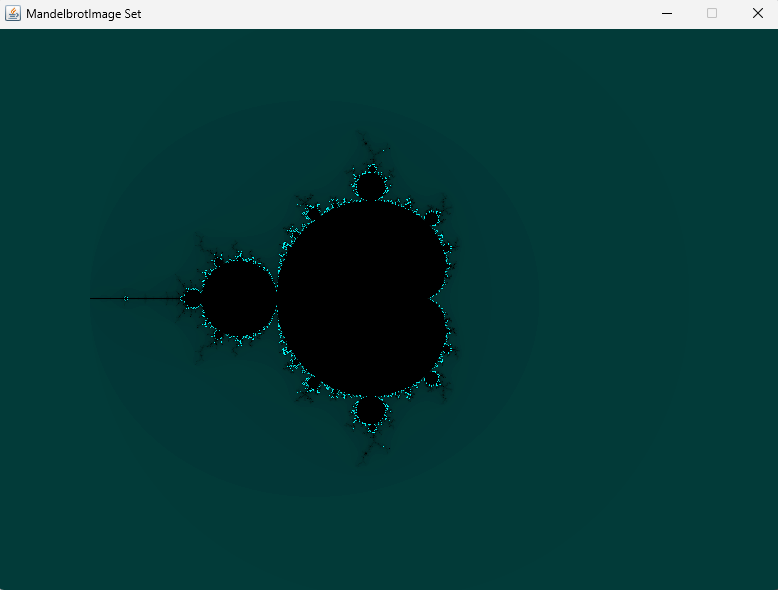
\includegraphics[width=1.0\textwidth]{./manedelbrot.png}
\caption{Wynik programu}
\end{figure}
\section*{Porównanie w zależności od implementacji Executora}
\label{sec:orgbdd40cc}
Metoda \texttt{run} pozwala nam na przetestowanie różnych implementacji executorów.
Parametr \texttt{MAX\_ITER} ustawiamy na \(200 000\), aby zwiększyć czas obliczeń.
Kod został uruchomiony na komputerze ośmiordzeniowym.

Kod testujący:
\begin{Code}
\begin{Verbatim}
\color{EFD}\EFk{private} \EFt{record} \EFf{ExecutorWithDesc}\EFrda{(}\EFt{ExecutorService} \EFv{executor}, \EFt{String} \EFv{desc}\EFrda{)} \EFrda{\{}
\EFrda{\}}
\EFk{public} \EFk{static} \EFt{void} \EFf{main}\EFrda{(}\EFt{String}\EFrdb{[}\EFrdb{]} \EFv{args}\EFrda{)} \EFrda{\{}
        \EFt{var} \EFv{executors} = List.of\EFrdb{(}
                \EFk{new} \EFt{ExecutorWithDesc}\EFrdc{(}Executors.newSingleThreadExecutor\EFrdd{(}\EFrdd{)},
                             \EFs{"Single thread"}\EFrdc{)},
                \EFk{new} \EFt{ExecutorWithDesc}\EFrdc{(}Executors.newFixedThreadPool\EFrdd{(}\EFhn{1}\EFrdd{)},
                             \EFs{"Fixed thread pool (1 threads)"}\EFrdc{)},
                \EFk{new} \EFt{ExecutorWithDesc}\EFrdc{(}Executors.newFixedThreadPool\EFrdd{(}\EFhn{2}\EFrdd{)},
                             \EFs{"Fixed thread pool (2 threads)"}\EFrdc{)},
                \EFk{new} \EFt{ExecutorWithDesc}\EFrdc{(}Executors.newFixedThreadPool\EFrdd{(}\EFhn{4}\EFrdd{)},
                             \EFs{"Fixed thread pool (4 threads)"}\EFrdc{)},
                \EFk{new} \EFt{ExecutorWithDesc}\EFrdc{(}Executors.newFixedThreadPool\EFrdd{(}\EFhn{8}\EFrdd{)},
                             \EFs{"Fixed thread pool (8 threads)"}\EFrdc{)},
                \EFk{new} \EFt{ExecutorWithDesc}\EFrdc{(}Executors.newFixedThreadPool\EFrdd{(}\EFhn{16}\EFrdd{)},
                             \EFs{"Fixed thread pool (16 threads)"}\EFrdc{)},
                \EFk{new} \EFt{ExecutorWithDesc}\EFrdc{(}Executors.newFixedThreadPool\EFrdd{(}\EFhn{32}\EFrdd{)},
                             \EFs{"Fixed thread pool (32 threads)"}\EFrdc{)},
                \EFk{new} \EFt{ExecutorWithDesc}\EFrdc{(}Executors.newWorkStealingPool\EFrdd{(}\EFrdd{)},
                             \EFs{"Work stealing pool (parallelism = \#CPU)"}\EFrdc{)},
                \EFk{new} \EFt{ExecutorWithDesc}\EFrdc{(}Executors.newWorkStealingPool\EFrdd{(}\EFhn{1}\EFrdd{)},
                             \EFs{"Work stealing pool (parallelism = 1)"}\EFrdc{)},
                \EFk{new} \EFt{ExecutorWithDesc}\EFrdc{(}Executors.newWorkStealingPool\EFrdd{(}\EFhn{4}\EFrdd{)},
                             \EFs{"Work stealing pool (parallelism = 4)"}\EFrdc{)},
                \EFk{new} \EFt{ExecutorWithDesc}\EFrdc{(}Executors.newWorkStealingPool\EFrdd{(}\EFhn{8}\EFrdd{)},
                             \EFs{"Work stealing pool (parallelism = 8)"}\EFrdc{)},
                \EFk{new} \EFt{ExecutorWithDesc}\EFrdc{(}Executors.newWorkStealingPool\EFrdd{(}\EFhn{16}\EFrdd{)},
                             \EFs{"Work stealing pool (parallelism = 16)"}\EFrdc{)},
                \EFk{new} \EFt{ExecutorWithDesc}\EFrdc{(}Executors.newWorkStealingPool\EFrdd{(}\EFhn{32}\EFrdd{)},
                             \EFs{"Work stealing pool (parallelism = 32)"}\EFrdc{)},
                \EFk{new} \EFt{ExecutorWithDesc}\EFrdc{(}Executors.newCachedThreadPool\EFrdd{(}\EFrdd{)},
                             \EFs{"Cached thread pool"}\EFrdc{)}
        \EFrdb{)};

        System.out.println\EFrdb{(}\EFs{"ExecutorName,Time"}\EFrdb{)};
        \EFk{for} \EFrdb{(}\EFt{var} \EFv{executor} : executors\EFrdb{)} \EFrdb{\{}
            \EFt{var} \EFv{start} = System.nanoTime\EFrdc{(}\EFrdc{)};
            \EFt{int}\EFrdc{[}\EFrdc{]}\EFrdc{[}\EFrdc{]} \EFv{image} = run\EFrdc{(}executor.executor, 200\_000, \EFhn{600}, \EFhn{800}\EFrdc{)};
            \EFt{var} \EFv{end} = System.nanoTime\EFrdc{(}\EFrdc{)};

            \EFt{var} \EFv{timeMs} = \EFrdc{(}end - start\EFrdc{)} / 1\_000\_000;
            System.out.println\EFrdc{(}executor.desc + \EFs{","} + timeMs\EFrdc{)};
        \EFrdb{\}}

\EFrda{\}}
\end{Verbatim}
\end{Code}

Wynik programu:
\begin{tcolorbox}
\begin{Verbatim}
ExecutorName,Time
Single thread,34914
Fixed thread pool (1 threads),33507
Fixed thread pool (2 threads),18269
Fixed thread pool (4 threads),8531
Fixed thread pool (8 threads),4420
Fixed thread pool (16 threads),4331
Fixed thread pool (32 threads),4320
Work stealing pool (parallelism = #CPU),4471
Work stealing pool (parallelism = 1),33299
Work stealing pool (parallelism = 2),17205
Work stealing pool (parallelism = 4),8501
Work stealing pool (parallelism = 8),4413
Work stealing pool (parallelism = 16),4380
Work stealing pool (parallelism = 32),4325
Cached thread pool,4381
\end{Verbatim}


\end{tcolorbox}Używając tych danych możemy stworzyć wykresy porównujące te implementacje.
\newpage

\begin{figure}[H]
\centering
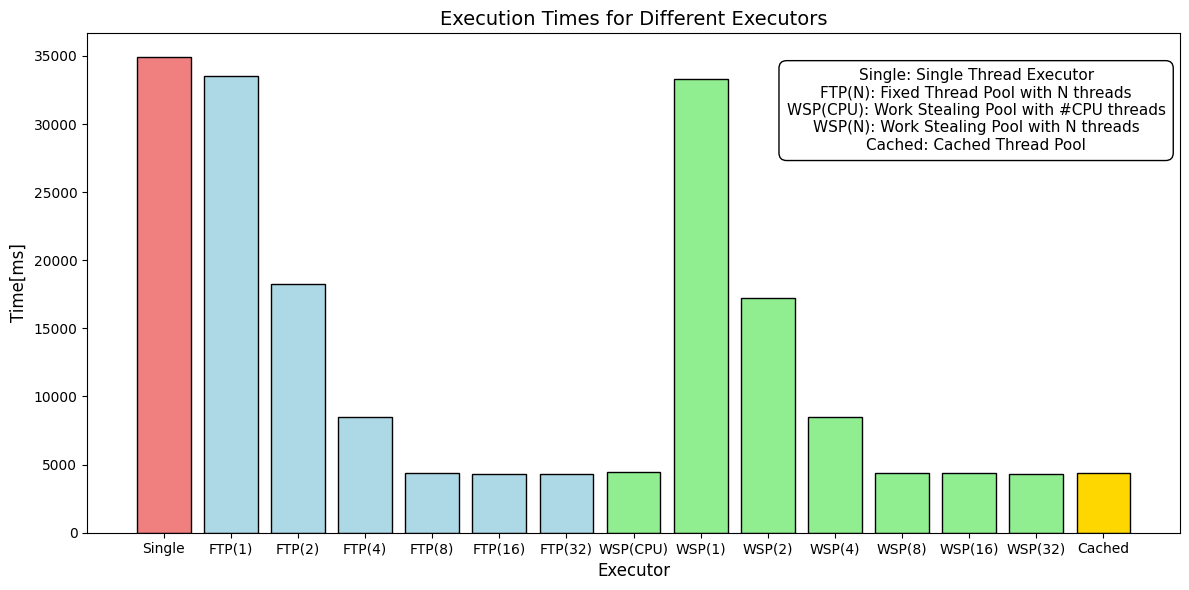
\includegraphics[width=0.85\textwidth]{./exec.png}
\caption{Czasy wykonania obliczeń w zależności od użytego executora.}
\end{figure}


\begin{figure}[H]
\centering
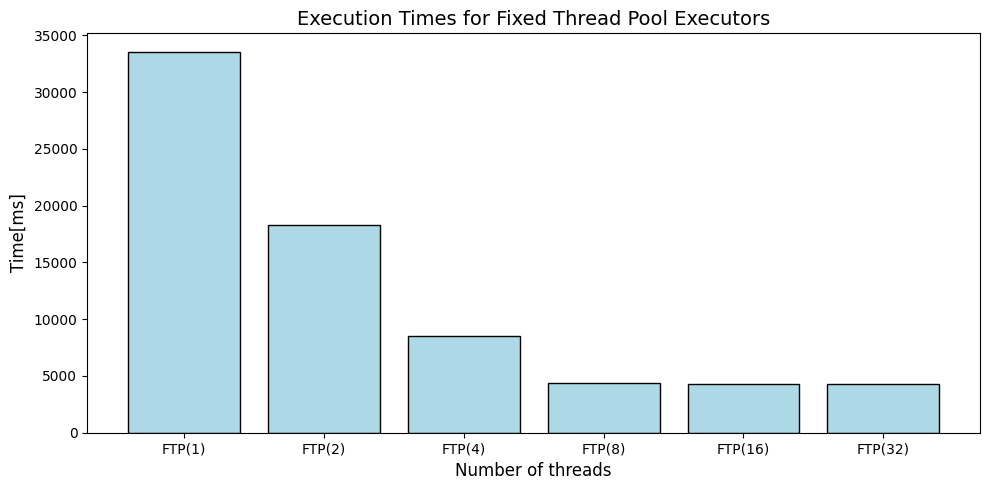
\includegraphics[width=0.85\textwidth]{./fixed.png}
\caption{Czasy wykonania obliczeń w zależności od ilości wątków dla executora o stałej liczbie wątków.}
\end{figure}


\begin{figure}[H]
\centering
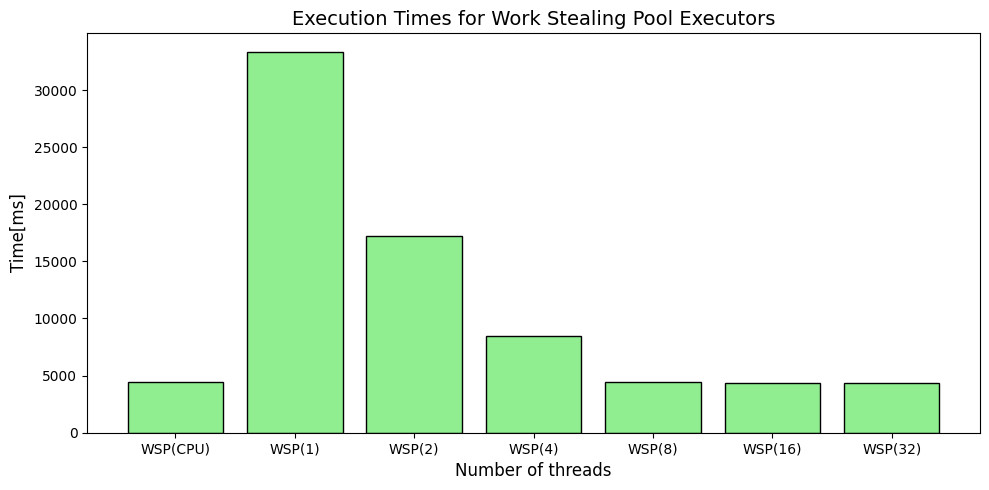
\includegraphics[width=0.85\textwidth]{./steal.png}
\caption{Czasy wykonania obliczeń w zależności od ilości wątków dla executora z mechanizmem "kradzieży pracy".}
\end{figure}
\section*{Wnioski}
\label{sec:org65c3935}


Analizując wykresy dochodzimy do następujących wniosków:
\begin{itemize}
\item Czas wykonania dla \texttt{SingleThreadExecutor} jest, według oczekiwań,
najdłuższy. Jest to spowodowane tym, że zadania są wykonywane sekwencyjnie.
Nasz program nie jest w stanie zrównoleglić obliczeń i wykorzystać
wielu rdzeni procesora.
\item Również wedle oczekiwań executory z pulami wątków jak \texttt{FixedThreadPoolExecutor} i
\texttt{WorkStealingPool} w przypadku podania ilości wątków równej 1 ''degradują'' się
 do \texttt{SingleThreadExecutor} jeżeli chodzi o czas wykonania.
\item \texttt{SingleThreadExecutor} nie jest dobry wyborem gdy mamy do wykonania
mnóstwo obliczeń, które można zrównoleglić.
\item Zarówno w przypadku \texttt{FixedThreadPoolExecutor} jak i \texttt{WorkStealingPoolExecutor},
czas wykonania maleje wraz ze wzrostem ilości wątków. Zwięszkenie
dwukrotne ilości wątków powoduje zmniejszenie czasu wykonania o około 50\%.
Oczywiście do pewnego momentu(8 wątków) po czym zyski ze zwiększenia ilości
wątków są w zasadzie żadne, bo użyty procesor
ma jedynie 8 rdzeni. Czasy wykonania dla obu executorów są bardzo zbliżone,
co oznacza, że obsługa ''kradzieży pracy'' nie wpływa znacząco na czas wykonania.
\item \texttt{CachedThreadPoolExecutor}, charakteryzuje się brakiem stałej liczby wątków.
Executor tworzy nowe wątki w miarę potrzeby, a wątki nieaktywne przez pewien
czas są usuwane. W naszym przypadku, czas wykonania jest zbliżony do
\texttt{WorkStealingPoolExecutor} i \texttt{FixedThreadPoolExecutor} z 8 wątkami.
\item Robiąc ten eksperyment oczekiwałem, że najszybszym wyborem będzie
\texttt{FixedThreadPoolExecutor} z 8 wątkami, z racji prostoty oraz
liczby wątków równych liczbie rdzeni procesora. Jednakże, równie
dobrze radzi sobie \texttt{WorkStealingPoolExecutor} jak i \texttt{CachedThreadPoolExecutor}.
Zaletą \texttt{WorkStealingPoolExecutor} jest to, że nie musimy podawać ilości wątków,
bo automatycznie dostosowuje się do liczby rdzeni procesora.
Oczywiście ''kradzież pracy'' również jest zaletą w przypadku, gdy
niektóre zadania są bardziej złożone niż inne.
\end{itemize}
\section*{Bibliografia}
\label{sec:orgf69cdeb}
\begin{itemize}
\item \href{https://www.baeldung.com/java-executor-service-tutorial}{Baeldung - Java Executor Service Tutorial}
\item \href{https://docs.oracle.com/javase/8/docs/api/?java/util/concurrent/Executors.html}{Dokumentacja pakietu Executors}
\end{itemize}
\end{document}
